\documentclass[12pt]{article}
\usepackage[utf8]{inputenc}
\usepackage[english]{babel}
\usepackage{amsmath, amsthm, amssymb, amsfonts}
\usepackage[top = 3in, left = 1in, right = 1in]{geometry}
\usepackage{hyperref, cleveref}
\hypersetup{
	colorlinks=true,
	linkcolor=blue,
	filecolor=magenta,      
	urlcolor=blue,
}
\usepackage{tcolorbox}
\usepackage{bm}


% FOR TIKZ
\usepackage{tikz}
\usetikzlibrary{arrows,arrows.meta, shapes.geometric}




% DEFINE NEW COMMANDS AND ENVIRONMENTS
\newcommand{\R}{\mathbb{R}}
\newcommand{\C}{\mathbb{C}}
\newcommand{\N}{\mathbb{N}}
\newcommand{\Q}{\mathbb{Q}}
\newcommand{\Z}{\mathbb{Z}}
\newcommand{\E}{\mathbb{E}}
\newcommand{\Var}{\mathbb{V}\text{ar}}


\newcommand{\HRule}{\rule{\linewidth}{0.5mm}} % Defines a new command for the horizontal lines, change thickness here


% DEFINE A PROBLEM Environment
\theoremstyle{definition}
\newtheorem*{prb}{Problem}
\newenvironment{problem}{
\begin{tcolorbox}[colback=blue!5!white,colframe=blue!75!black, parbox = true] \begin{prb}  }{\end{prb}\end{tcolorbox} }
\newenvironment{answer}{\textit{Solution: }\quad }{ \hfill $\blacksquare$}
\newtheorem{claim}{Claim}




\begin{document}


% TITLE PAGE
%%%%%%%%%%%%%%%%%%%%%%%%%%%%%%%%%%%%%%%%%%%%%%%%%%%%%%
\begin{titlepage}
    
\centering
\textsc{\LARGE Indian Statistical Institute, Kolkata}\\[1.5cm] % Name of your university/college
\textsc{\Large Measure Theoretic Probability}\\[0.5cm] % Major heading such as course name
\textsc{\large Semestral Assignment: Second Semester 2019-2020}\\[0.5cm] % Minor heading such as course title

\HRule \\[0.4cm]
\large \textbf{Subhrajyoty Roy}\\
\large \textbf{Roll:  MB1911}\\
\HRule \\[1.5cm]
\normalsize \today

\end{titlepage}


\tableofcontents
\clearpage


% CONTENT FROM HERE
%%%%%%%%%%%%%%%%%%%%%%%%%%%%%%%%%%%%%%%%%%%%%%%%%%
\newgeometry{margin = 1in}

\section{Problem 1}

\begin{problem}
	Let, $\mathcal{C} = \left\{ A \subseteq \R : A \text{ is countable or } \R \backslash A \text{ is countable} \right\}$ be the countable-cocountable $\sigma$-field on $\R$. Let, $f : \R \rightarrow \R$ be a function. Show that, $\forall B \in \mathcal{B}_{\R}$, $f^{-1}(B) \in \mathcal{C}$ iff there exists a countable set $A \subset \R$ and $c \in \R$ such that, $f(x) = c, \forall x \notin A$. 
\end{problem}

\begin{answer}
	I shall first proceed with the if part and then the only if part.

	\textbf{\underline{If part:}}

	Here, it is given that there exists a countable set $A \subset \R$ and $c \in \R$ such that, $f(x) = c$ for any $x \notin A$. Therefore, for any real $x \in \R$, either $f(x) = c$ or $x \in A$, i.e. $\R = A \cup f^{-1}(\left\{ c \right\})$, i.e. $f(\R) = A^\ast \cup \left\{ c \right\}$ where $A^\ast = f(A) = \left\{ f(x) : x \in A \right\}$.

	Now choose any set $B \in \mathcal{B}_{\R}$.
	\begin{enumerate}
		\item If $c \in B$, then $f^{-1}(B) \supseteq f^{-1}(\left\{ c \right\}) = \R \backslash A$. Therefore, $\R \backslash f^{-1}(B) \subseteq A$, and as $A$ is countable, $\R \backslash f^{-1}(B)$ is countable as well. This shows $f^{-1}(B) \in \mathcal{C}$ as it is cocountable.
		\item If $c \notin B$, then 
		$$f^{-1}(B) = f^{-1}(B \cap A^\ast) \subseteq f^{-1}(A^\ast) = A$$
		Hence, $f^{-1}(B)$ would be countable and thereby belongs to $\mathcal{C}$. 
	\end{enumerate}


	\textbf{\underline{Only If:}}

	Here, it is assumed that, for any $B \in \mathcal{B}_{\R}$, $f^{-1}(B) \in \mathcal{C}$, i.e. either $f^{-1}(B)$ or its complement is countable. Since, $f^{-1}(B^c) = (f^{-1}(B))^c$, hence either $B$ or $B^c$ must have its pre-image set as a countable set.

	\begin{claim}
		\label{remark:1-1}
		For all $B \in \mathcal{B}_{\R}$, either $f^{-1}(B)$ or $f^{-1}(B^c)$ is countable.
	\end{claim}

	Let us consider a countable cover for the whole real line,

	$$\R = \cup_{n = -\infty}^{\infty} (n, n+1]$$

	Clearly, as $f$ is a function, $f^{-1}(\R)$ is uncountable. Since, $f^{-1}(\R) = \cup_{n = -\infty}^{\infty} f^{-1}( (n, n+1] )$, which is a countable union, atleast one of the set among the ones above must be uncountable in size. Without loss of generality, assume, $(0, 1]$ be one such set so that, $f^{-1}((0, 1])$ is uncountable.
	
	Now, it will be shown that it is only such set whose pre-image is uncountable. By the \cref{remark:1-1} made earlier, it is obvious once we take $B = (0, 1]$ and $B^c = \cup_{n = -\infty \\ n \neq 0}^{\infty} (n, n+1]$ whose preimage must be countable, and hence each of pre-image $f^{-1}((n, n+1]) \subseteq f^{-1}(B^c)$ is countable for any $n \in \Z \backslash \left\{ 0 \right\}$.

	Let, $a_1 = 0, b_1 = 1$. Then, the closed interval $[a_1, b_1]$ has its pre-image uncountable (as it contains $(0, 1]$). Now, we consider a division of the interval into two equal parts, $[0, 1/2]$ and $(1/2, 1]$, and since $f^{-1}([0, 1]) = f^{-1}([0, 1/2]) \cup f^{-1}((1/2, 1])$. Again by exactly same logic as before exactly one of these pre-images is uncountable. We call this $[a_2, b_2]$. (If the set is not closed then we add the endpoints to it so that it becomes closed and still retain the above property.) We apply this step inductively to obtain a sequence of nested closed intervals, $I_1 \supset I_2 \supset I_3 \dots \subset I_m \dots$, where $I_m = [a_m, b_m]$. Also, since we are making these intervals of half length at each step, $(b_m - a_m) = 2^{-(m-1)} \rightarrow 0$, as $m \rightarrow \infty$. 

	Therefore, by Cantor's Intersection theorem\footnote{\textbf{Statement:} If $C_1, \supseteq C_2 \supseteq \dots C_n \subseteq \dots$ be a sequence of nested closed bounded intervals in $\R$ such that $\lim_{n \rightarrow \infty}\text{Diam}(C_n) \rightarrow 0$, then $\cap_{n=1}^{\infty}C_n$ contains exactly one point}, there exists exactly a single point $c \in R$ such that, $\cap_{m = 1}^{\infty} I_m = \left\{ c \right\}$. Due to the repeated application of \cref{remark:1-1} and the choice of the nested closed intervals $I_m$'s, for the complementary sets we have, $f^{-1}(\R \backslash I_1), f^{-1}(I_1 \backslash I_2), f^{-1}(I_2 \backslash I_3), \dots$ are countable sets. Since,

	$$
	\left(\cap_{m = 1}^{\infty} I_m \right)^c
	= \cap_{m=1}^{\infty} I_m^c
	= (\R \backslash I_1) \cup (I_1 \backslash I_2) \cup (I_2 \backslash I_3) \cup \dots
	$$

	Therefore,

	$$f^{-1}(\left\{ c \right\}^c) = f^{-1}(\left(\cap_{m = 1}^{\infty} I_m \right)^c) = f^{-1}(\R \backslash I_1) \cup \cup_{n = 1}^{\infty} f^{-1}(I_n \backslash I_{n+1})$$

	which is a countable union of countable sets, and hence is countable. We call this set $A$. Then clearly, for all $x \notin A$, $f(x) = c$, which was what we intended to show.
\end{answer}


\pagebreak
\section{Problem 2}

\begin{problem}
	Let, $a_0, a_n, b_n, n \geq 1$ be real numbers such that the series
	$$\dfrac{a_0}{2} + \sum_{n = 1}^{\infty} a_n \cos nx + \sum_{n = 1}^{\infty} b_n \sin nx$$
	converges absolutely on a set of positive Lebesgue measure. In other words, Lebesgue measure of $E = \left\{ x\in[-\pi, \pi] : \sum_{n=1}^{\infty} \vert a_n \vert \vert \cos nx \vert + \sum_{n=1}^{\infty} \vert b_n \vert \vert \sin nx \vert < \infty \right\}$ is positive. Show that, $\sum_{n=1}^{\infty} (\vert a_n \vert + \vert b_n \vert) < \infty$.

	\textbf{Note:} You would possibly need the following fact. If $f: [-\pi, \pi] \rightarrow \R$ be a bounded measurable function, then both $\int_{-\pi}^{\pi} f(x) \cos (nx) d\lambda(x)$ and $\int_{-\pi}^{\pi} f(x) \sin (nx) d\lambda(x)$ converge to zero as $n$ goes to infinity.
\end{problem}

\begin{answer}
	We have, $E = \left\{ x\in[-\pi, \pi] : \sum_{n=1}^{\infty} \vert a_n \vert \vert \cos nx \vert + \sum_{n=1}^{\infty} \vert b_n \vert \vert \sin nx \vert < \infty \right\}$ and it is given that $\lambda(E) > 0$, where $\lambda$ denotes the usual Lebesgue measure.

	Let, $F = \left\{ x \in [-\pi, \pi] : \sum_{n=1}^{\infty} \vert a_n \cos nx + b_n \sin nx \vert < \infty \right\}$. Since, by triangle inequality;

	$$\vert a_n \cos nx + b_n \sin nx \vert < \vert a_n \vert \vert \sin nx \vert + \vert b_n \vert \vert \cos nx \vert$$

	Hence, $E \subseteq F$ and, therefore, $\lambda(F) \geq \lambda(E) > 0$, and obviously, $F \subseteq [-\pi, \pi]$ implies $\lambda(F)\leq \lambda([-\pi, \pi]) = 2\pi$. Now, 

	\begin{align*}
		a_n \cos nx + b_n \cos nx
		& = r_n \left[ \dfrac{a_n}{r_n} \cos nx + \dfrac{b_n}{r_n} \sin nx \right], \quad \text{where } r_n = \sqrt{(a_n^2 + b_n^2)}\\
		& = r_n \left[ \sin \theta_n \cos nx + \cos \theta_n \sin nx \right], \quad \text{ where } \theta_n = \tan^{-1}\left(\dfrac{b_n}{a_n} \right)\\
		& = r_n \sin (\theta_n + nx)\\
	\end{align*}

	Therefore, 

	$$F = \left\{ x \in [-\pi, \pi] : \sum_{n=1}^{\infty} r_n \vert \sin(\theta_n + nx) \vert < \infty \right\}$$

	Now, since $\vert \sin(\theta_n + nx) \vert \leq 1$, we try to bound the series so that, $\sum_{n=1}^{\infty} r_n$ can be bounded.

	For this reason, we consider the sets $F_m = \left\{ x \in F : \sum_{n=1}^{\infty} r_n \vert \sin (\theta_n + nx) \vert < m \right\}$. Clearly, the sets $F_m \uparrow F$, and hence the Lebesgue measure $\lambda(F_m) \uparrow \lambda(F)$, provided that $F_m$'s  and $F$ are measurable, which we state as a claim.

	\begin{claim}
		The sets $F_m = \left\{ x \in F : \sum_{n=1}^{\infty} r_n \vert \sin (\theta_n + nx) \vert < m \right\}$ are measurable for any $m \in \N$. Also, the set $F = \left\{ x \in [-\pi, \pi] : \sum_{n=1}^{\infty} r_n \vert \sin(\theta_n + nx) \vert < \infty \right\}$ is measurable.
		\label{claim:2-1}
	\end{claim}

	\begin{proof}
		To prove the claim, let us consider a function $h: \R \rightarrow [0, \infty]$ given by;

		$$h(x) = \sum_{n=1}^{\infty} r_n \vert \sin (\theta_n + nx) \vert$$

		And let, $h_m(x)$ denotes the partial sums, namely $h_m(x) = \sum_{n=1}^{m} r_n \vert \sin (\theta_n + nx) \vert$. Note that, $\sin(\theta_n + nx)$ is measurable being a continuous function of $x$, and so is its absolute value. Being a finite sum of such terms, $h_m$ is also a measurable function. Also, $h_m$ is non-negative for each $m \geq 1$, $h_m$ are non-decreasing (with respect to $m$) and $h_m \uparrow h$. Hence the function $h$ is also measurable. 

		Finally, note that $F_m = F \cap h^{-1}((-\infty, m))$, which is measurable provided that $F$ is measurable.

		However,

		$$F = \left\{ x\in [-\pi, \pi] : \lim_{m \rightarrow \infty} h_m(x) < \infty \right\}$$

		which is measurable due to Proposition 3.2.5 of the notes.\footnote{\textbf{Statement of the Proposition:} Let $(\Omega, \mathcal{G})$ be a measurable space and $X_n : \Omega \rightarrow \R$ be sequence of real valued random variables. Then $A = \left\{ w \in \Omega : \lim_{n} X_n(w) < \infty \right\}$ is a measurable set.}
	\end{proof}

	Now, due to \cref{claim:2-1}, $\lambda(F_m) \uparrow \lambda(F)$, and since, $\lambda(F) > 0$, this means there exists $M$ such that, $\forall m \geq M$, $\lambda(F_m) > 0$. Therefore,

	\begin{equation}
		\label{eqn:2-1}
		\begin{split}
		\int_{F_M} \sum_{n = 1}^{\infty} r_n \vert \sin (\theta_n + nx) \vert d\lambda
		& = \int_{\R} \bm{1}_{F_M} \sum_{n = 1}^{\infty} r_n \vert \sin (\theta_n + nx) \vert d\lambda,\\
		& \qquad \qquad \text{ where } \bm{1}_A \text{ is the indicator function of set } A \\
		& \leq \int_{\R} \bm{1}_{F_M} M d\lambda, \quad \text{ as } \forall x \in F_M, \text{ the series is bounded by } M\\
		& \qquad \qquad \text{ and the rest follows from monotonicity of integral}\\
		& = M \int_{F_M} d\lambda \quad \text{ by linearity of integral}\\
		& = M \lambda(F_M)
		\end{split}
	\end{equation}

	On the other hand, 

	\begin{align*}
		\vert \sin (\theta_n + nx) \vert 
		& \geq \sin^2 (\theta_n + nx), \quad \text{ since } \vert \sin (\theta_n + nx) \vert \leq 1\\
		& = \dfrac{1}{2} \left[ 1 - \cos(2\theta_n + 2nx) \right]\\
		& = \dfrac{1}{2} - \dfrac{1}{2} \cos(2\theta_n)\cos(2nx) + \dfrac{1}{2} \sin(2\theta_n)\sin(2nx)\\
	\end{align*}

	Now, 

	\begin{equation}
		\begin{split}
		\int_{F_M} \vert \sin(\theta_n + nx) \vert d\lambda 
		& \geq \int_{F_M}  \left[\dfrac{1}{2} - \dfrac{1}{2} \cos(2\theta_n)\cos(2nx) + \dfrac{1}{2} \sin(2\theta_n)\sin(2nx)\right] d\lambda\\
		& \qquad \qquad \text{ by monotonicity of integral}\\
		& = \dfrac{\lambda(F_M)}{2} - \dfrac{1}{2} \cos(2\theta_n) \int_{F_M} \cos(2nx) d\lambda + \dfrac{1}{2} \sin(2\theta_n) \int_{F_M} \sin(2nx) d\lambda
		\end{split}
		\label{eqn:2-2}
	\end{equation}
	
	Note that, 

	$$\int_{F_M}\cos(2nx) d\lambda(x) = \int_{-\pi}^{\pi} \bm{1}_{F_M}(x) \cos(2nx) d\lambda(x)$$

	where, $\bm{1}_{F_M}(x) = 1$ if $x \in F_M$, $0$ otherwise. Clearly, by the note given in the question, as $n \rightarrow \infty$, the above integral converges to zero, as $\bm{1}_{F_M}(x)$ is a bounded measurable function since $F_M$ is a measurable set.

	Similarly, $\int_{F_M} \sin(2nx) d\lambda(x) \rightarrow 0$ as $n \rightarrow \infty$. Also, since $\cos(2\theta_n)$ is a bounded sequence of real numbers, combining with above yields, $\dfrac{1}{2} \cos(2\theta_n) \int_{F_M} \cos(2nx) d\lambda \rightarrow 0$ as $n \rightarrow \infty$. By similar argument, we also have, $\dfrac{1}{2} \sin(2\theta_n) \int_{F_M} \sin(2nx) d\lambda \rightarrow 0$ as well.

	Therefore, by applying the limit $n \rightarrow \infty$ on \cref{eqn:2-2}, we obtain the existence of $n_0 \in \N$ such that for all $n \geq n_0$, 

	$$\int_{F_M} \vert \sin(\theta_n + nx)\vert d\lambda \geq \dfrac{\lambda(F_M)}{3}$$

	as $\dfrac{\lambda(F_M)}{3} < \dfrac{\lambda(F_M)}{2}$ since $\lambda(F_M) > 0$. Therefore,

	\begin{equation}
		\begin{split}
			\int_{F_M} \sum_{n = n_0}^{\infty} r_n \vert \sin(\theta_n + nx) \vert d\lambda
			& = \sum_{n = n_0}^{\infty} r_n \int_{F_M} \vert \sin(\theta_n + nx) \vert d\lambda\\
			& \qquad \qquad \text{ can interchange the sum and the integral since}\\
			& \qquad \qquad \text{it is finite by \cref{eqn:2-1}}\\
			& \geq \sum_{n = n_0}^{\infty} r_n \dfrac{\lambda(F_M)}{3}
		\end{split}
		\label{eqn:2-3}
	\end{equation}

	Now combining \cref{eqn:2-1} and \cref{eqn:2-3}, we get that,

	$$\dfrac{\lambda(F_M)}{3} \sum_{n = n_0}^{\infty} r_n \leq \int_{F_M} \sum_{n = n_0}^{\infty} r_n \vert \sin(\theta_n + nx) \vert d\lambda \leq M \lambda(F_M)$$

	Since, $\lambda(F_M) > 0$, this yields;

	$$\sum_{n = 1}^{\infty} r_n \leq \sum_{n = 1}^{(n_0 -1)} r_n + M < \infty$$

	Finally, an application of QM-AM inequality yields, $\sqrt{2}\sqrt{a_n^2 + b_n^2} \geq (\vert a_n \vert + \vert b_n \vert)$. Thus,

	$$\sum_{n = 1}^{\infty} (\vert a_n \vert + \vert b_n \vert) \leq \sqrt{2}\sum_{n = 1}^{\infty} r_n < \infty$$
	
	This completes the proof of the result.

\end{answer}


\pagebreak
\section{Problem 3}
\begin{problem}
	Let, $X$ be a random variable having distribution function $F$. Show that, $\E(F(X))\geq 1/2$ with equality iff $F$ is continuous.
\end{problem}

\begin{answer}
	We denote the measure space associated with the random variable $X$ as $(\Omega, \mathcal{G}, \mu)$, where $\mu$ is the probability measure.

	Let us assume existence of two random variables $X_1$ and $X_2$ such that both of these random variables have the same distribution function $F$ as $X$.\footnote{Note that, independence of $X_1$ and $X_2$ are not assumed.} Let, $\mu$ be the probability measure associated with $X$, hence associated with $X_1$ and $X_2$ as well.

	Then,
	\begin{align*}
		\E(F(X))
		& = \E(F(X_1))\\
		& = \int_{-\infty}^{\infty} F(x_1) \mu(dx_1)\\
		& = \int_{-\infty}^{\infty} \int_{-\infty}^{x_1} \mu(dx_2) \mu(dx_1) \qquad \text{, since } F \text{ is distribution function of } X_2 \text{ also}\\
		& = \int_{\R^2} \bm{1}_{\left\{ (x_1, x_2) : x_2 \leq x_1 \right\} }(x_1, x_2) \mu(dx_2) \mu(dx_1) \qquad \text{ where } \bm{1}_A \text{ is the indicator function of } A \\
	\end{align*}

	Now in order to get a product probability measure in the product space, we extend these individual measures to a transition probability measure, simply as follows:

	Define, $\mu_{12}: \Omega \times \mathcal{G} \rightarrow [0, \infty]$ as $\mu_{12}(w, B) = \mu(B) \quad \forall B \in \mathcal{G}$. Then clearly,

	\begin{enumerate}
		\item For any $w \in \Omega$, $\mu_{12}(w, \cdot)$ is $\sigma$-finite as $\mu_{12}(w, \Omega) = \mu(\Omega) = 1 < \infty$.
		\item For any $B \in \mathcal{G}$, $\mu_{12}(\cdot, B) : \Omega \rightarrow [0, \infty]$ is measurable, as $\mu_{12}(\cdot, B) = \mu(B)$, the constant function which is trivially measurable.
	\end{enumerate}

	Now that we have $\mu_{12}$ as a transition measure, it is also easy to note that it is uniformly $\sigma$-finite. This is because, $\sup_{w \in \Omega} \mu_{12}(w, B) = \mu(B) \leq \mu(\Omega) = 1 < \infty$. 

	Hence, letting $S = \left\{ (x_1, x_2) : x_2 \leq x_1 \right\}$, an application of Fubini's theorem yields;

	$$\E(F(X)) = \int_{\R^2} \bm{1}_{S}(x_1, x_2) \mu(dx_2) \mu(dx_1) = \int_{\R^2} \bm{1}_{S}(x_1,x_2) \mu_{12}(x_1, dx_2) \mu(dx_1) = \lambda(S)$$

	where $\lambda(\cdot)$ is a $\sigma$-finite measure on the product space $\mathcal{G} \otimes \mathcal{G}$. Consequently, reversing the role of $x_1$ and $x_2$ in the order to integration, we could consider,

	$$\lambda(S) = \int_{\R^2} \bm{1}_{S}(x_1, x_2) \mu_{12}(x_2, dx_1) \mu(dx_2) = \int_{\R^2} \bm{1}_{S}(x_1, x_2) \mu(dx_1) \mu(dx_2)$$

	Therefore, finally we have;

	\begin{equation}
		\E(F(X)) = \int_{\R^2} \bm{1}_{\left\{ (x_1, x_2) : x_2 \leq x_1 \right\}}(x_1, x_2) \mu(dx_1) \mu(dx_2)
		\label{eqn:3-1}
	\end{equation}

	However, for all $(x_1, x_2) \in \R^2$ we have,

	\begin{equation}
		\bm{1}_{ \left\{ (x_1, x_2) : x_2 \leq x_1 \right\} }(x_1, x_2) +
		\bm{1}_{ \left\{ (x_1, x_2) : x_2 \geq x_1 \right\} }(x_1, x_2) -
		\bm{1}_{ \left\{ (x_1, x_2) : x_2 = x_1 \right\} }(x_1, x_2) = 1
		\label{eqn:3-2}
	\end{equation}

	Let us call the sets $\left\{ (x_1, x_2) : x_2 \geq x_1 \right\}$ and $\left\{ (x_1, x_2) : x_2 = x_1 \right\}$ as $T$ and $V$ respectively. Combining \cref{eqn:3-1} and \cref{eqn:3-2} together, it yields that;

	\begin{align*}
		\E(F(X))
		& = \int_{\R^2} \left( 1 - \bm{1}_T(x_1, x_2) + \bm{1}_V (x_1, x_2) \right) \mu(dx_1) \mu(dx_2)\\
		& = \int_{\R^2} \mu(dx_1) \mu(dx_2) - \int_{R^2} \bm{1}_T(x_1, x_2) \mu(dx_1) \mu(dx_2) + \int_{\R^2} \bm{1}_V(x_1, x_2) \mu(dx_1) \mu(dx_2)\\
		& = \int_{-\infty}^{\infty} \mu(\Omega) \mu(dx_2) - \int_{-\infty}^{\infty} \left(\int_{-\infty}^{x_2} \mu(dx_1)\right) \mu(dx_2) + \lambda(V)\\
		& = \int_{-\infty}^{\infty} \mu(dx_2) - \int_{-\infty}^{\infty} F(x_2) \mu(dx_2) + \lambda(V)\\
		& \qquad \qquad \text{since, } \mu(\Omega) = 1 \text{ and } \int_{-\infty}^{x_2} \mu(dx_1) = F(x_2)\\
		& = \mu(\Omega) - \E(F(X_2)) + \lambda(V)\\
		& = 1 + \lambda(V) - \E(F(X)) \quad \text{, as } X \text{ and } X_2 \text{ are identically distributed}\\
	\end{align*}

	Hence,

	$$2\E(F(X)) = 1 + \lambda(V) \geq 1$$

	as $\lambda(V)$ is a well defined measure (as noted earlier due to Fubini's theorem). Hence, $\E(F(X)) \geq \dfrac{1}{2}$.

	Note that, the equality holds if and only if $\lambda(V) = 0$. So, let us prove this concerning the equality case as two seperate parts.

	\begin{itemize}
		\item \textbf{If Part:} Suppose, $F$ is continuous. Then,
		
		\begin{claim}
			$F$ is uniformly continuous, since it is bounded between 0 and 1. 
		\end{claim}
		
		\begin{proof}
			A simple proof of this uniform continuity can be established by noting that, since $\lim_{x \rightarrow -\infty} F(x) = 0$ and $\lim_{x \rightarrow \infty} F(x) = 1$, for any given $\epsilon>0$, there exists $M$ large enough such that, $F(x) < \epsilon/2$ for any $x \leq (-M)$ and $(1 - F(x)) > \epsilon/2$, for any $x \geq M$. However, within the interval $[-M, M]$, $F$ restricted to this interval is a continuous function defined on a compact set, hence is uniformly continuous. Together, we have some $\delta$ such that, $\forall x, y \in \R$ such that, $\vert x - y\vert < \delta$;

		\begin{enumerate}
			\item If $x, y$ both are either in $(-\infty, -M)$ or in $(M, \infty)$, $\vert F(x) - F(y) \vert < \epsilon/2 + \epsilon/2 = \epsilon$.
			\item If $x, y$ are both in $[-M, M]$, then $\vert F(x) - F(y) \vert < \epsilon$ by uniform continuity of $F$ in the interval $[-M, M]$.
			\item If $x \in (-\infty, -M)$ and $y \in [-M, M]$ for example, then, 
			$$\vert F(x) - F(y) \vert \leq \vert F(x) \vert + \vert F(y) - F(-M) \vert + \vert F(-M) \vert < 2\epsilon$$ 
		\end{enumerate}

			which completes the argument for establishing the claim.
		\end{proof}

		Now, fix any $\epsilon> 0$. Since, $F$ is established to be uniformly continuous, we have some $\delta > 0$ such that for any $x \in \R$,
		
		\begin{equation}
			F\left( x + \delta \right) - F\left( x - \delta \right) < \epsilon
			\label{eqn:3-3}
		\end{equation}

		Therefore,

		\begin{align*}
			\lambda(V)
			& = \int_{\R^2} \bm{1}_V(x_1,x_2) \mu(dx_1) \mu(dx_2)\\
			& \leq \int_{\R^2} \bm{1}_{ \left\{ (x_1, x_2) : x_1 \in (x_2 - \delta, x_2 + \delta) \right\} }(x_1, x_2) \mu(dx_1) \mu(dx_2)\\
			& \qquad \qquad \text{ since, } \left\{ (x_1, x_2) : x_1 \in (x_2 - \delta, x_2 + \delta) \right\} \supseteq V\\
			& = \int_{-\infty}^{\infty} \left( F(x_2 + \delta) - F(x_2 - \delta) \right) \mu(dx_2)\\
			& \leq \epsilon \int_{-\infty}^{\infty} \mu(dx_2) \qquad \text{because of \cref{eqn:3-3}}\\
			& = \epsilon\qquad \text{since, } \mu(\Omega) = 1
		\end{align*}

		Since, $\epsilon$ is arbitrary, $\lambda(V) = 0$, and consequently the equality holds, i.e. $\E(F(X)) = \dfrac{1}{2}$.
		
		\item \textbf{Only If part:} Suppose, $\lambda(V) = 0$. We need to show that $F$ is continuous. 
		
		For the sake of contradiction, assume that $F$ is not continuous. Since by definition of distribution function, $F$ is right continuous everywhere, hence there must exist $x_0 \in \R$ such that, $\displaystyle\lim_{x \rightarrow x_0 -} F(x) < F(x_0)$. Hence,
		
		\begin{align*}
			\lambda(V)
			& = \int_{\R^2} \bm{1}_V(x_1, x_2) \mu(dx_1) \mu(dx_2)\\
			& \geq \int_{\R^2} \bm{1}_{ \left\{ (x_1, x_2): x_1 = x_2 = x_0 \right\} }(x_1, x_2)\mu(dx_1) \mu(dx_2)\\
			& \qquad \qquad \text{ since, } V \subseteq \left\{ (x_1, x_2): x_1 = x_2 = x_0 \right\}\\
			& = \int_{\R^2} \bm{1}_{ \left\{ (x_1, x_2): x_1 = x_0\right\} }(x_1, x_2) \bm{1}_{ \left\{ (x_1, x_2): x_2 = x_0\right\} }(x_1, x_2)\mu(dx_1) \mu(dx_2)\\
			& = \int_{-\infty}^{\infty} \mu(x_0) \bm{1}_{ \left\{ (x_1, x_2): x_2 = x_0\right\} }(x_1, x_2)\mu(dx_2)\\
			& = \mu(x_0) \int_{-\infty}^{\infty} \bm{1}_{ \left\{ (x_1, x_2): x_2 = x_0\right\} }(x_1, x_2)\mu(dx_2)\\
			& = (\mu(x_0))^2 \\
			& = \left( F(x_0) - \lim_{x \rightarrow x_0 -} F(x) \right)^2 > 0\\
		\end{align*}

		contradicting the fact that we assumed $\lambda(V) = 0$. Hence, it must be the case that $F$ is continuous.
	\end{itemize}

	This completes the proof for the equality case.

\end{answer}

\pagebreak
\section{Problem 4}
\begin{problem}
	Let, $X$ be a random variable such that $\E(X^2) < \infty$. Show that the characteristic function of $X$ is twice differentiable.
\end{problem}

\begin{answer}

	Let, $\phi(t) = \E(e^{itX})$ be the characteristic function of $X$, where $i$ is the complex number such that $(i^2 + 1) = 0$. Before proceeding with the main proof, we start by establishing two claims.

	\begin{claim}
		\label{claim:4-1}
		$$\lim_{h \rightarrow 0} \dfrac{e^{ihx} - 1}{h} = ix$$
	\end{claim}

	\begin{proof}
		The proof of this claim follows simply from the Taylor series expansion of $e^z$ for any complex number $z$. Hence,

		\begin{align*}
			\lim_{h \rightarrow 0} \dfrac{e^{ihx} - 1}{h}
			& = \lim_{h \rightarrow 0} \dfrac{ \sum_{k=0}^{\infty}\dfrac{(ihx)^k}{k!} - 1}{h}\\
			& = \lim_{h \rightarrow 0} \dfrac{1}{h} \sum_{k = 1}^{\infty} \dfrac{(ihx)^k}{k!}\\
			& = ix + \lim_{h \rightarrow 0} \sum_{k = 2}^{\infty} \dfrac{(ix)^k h^{(k-1)} }{k!}\\
			& = ix
		\end{align*}

		since, the later power series is continuous at $h = 0$ and takes value $0$ at $h = 0$.
	\end{proof}

	\begin{claim}
		\label{claim:4-2}
		If $x \in \R$, then $\vert e^{ix} - 1 \vert \leq \vert x \vert$.
	\end{claim}

	\begin{proof}
		If we consider the function $f(x) = e^{ix}$, then due to the above \cref{claim:4-1}, we have;

		$$\lim_{h \rightarrow 0} \dfrac{e^{i(x+h)} - e^{ix}}{h} = e^{ix} \lim_{h \rightarrow 0} \dfrac{e^{ih} - 1}{h} = ie^{ix}$$

		Therefore, for $x \geq 0$, we have;

		$$
		\vert e^{ix} - 1 \vert
		= \left\vert \int_{0}^{x} ie^{iu} du \right\vert
		\leq \int_{0}^{x} \vert ie^{iu} \vert du
		= \int_{0}^{x} du = x
		$$

		For $x < 0$, $\vert e^{ix} - 1 \vert = \vert e^{ix} \vert \vert 1 - e^{-ix} \vert = \vert e^{-ix} - 1 \vert \leq (-x)$

		Together, we have $\vert e^{ix} - 1 \vert \leq \vert x \vert$.
	\end{proof}
	
	Note that,

	\begin{align*}
		\dfrac{\phi(t+h) - \phi(t)}{h}
		& = \dfrac{\E(e^{i(t+h)X}) - \E(e^{itX})}{h}\\
		& = \int \dfrac{(e^{i(t+h)x} - e^{itx})}{h} dP\\
		& = \int e^{itx}\dfrac{(e^{ihx} - 1)}{h} dP\\
		& = \E \left( e^{itX}\dfrac{(e^{ihX} - 1)}{h} \right)
	\end{align*}

	Now, due to \cref{claim:4-2}, 

	$$
	\left\vert e^{itX}\dfrac{(e^{ihX} - 1)}{h} \right\vert 
	= \vert e^{itX} \vert \left\vert \dfrac{(e^{ihX} - 1)}{h} \right\vert
	\leq \vert hX \vert
	\leq \vert X \vert
	$$

	if $\vert h \vert \leq 1$. Since, $h \rightarrow 0$, this is possible to ensure at the limiting stage. Turning to the integral, we see that $e^{itx}\dfrac{(e^{ihx} - 1)}{h} \rightarrow ixe^{itx}$ as $h \rightarrow 0$, the integrand is bounded by $\vert X \vert$ for small $h$, and since $\E(X^2) < \infty$, $\E(\vert X \vert) < \infty$ as well, since by Holder's inequality, $\E(\vert X\vert) < \E(X^2)^{1/2} < \infty$. Therefore, by Dominated Convergence Theorem, 

	$$
	\phi'(t) = \lim_{h \rightarrow 0}\dfrac{\phi(t+h) - \phi(t)}{h}
	= \E(iX e^{itX}) 
	$$

	Now, proceeding similarly with this $\phi'(t)$ as starting point, we note that,

	\begin{align*}
		\dfrac{\phi'(t+h) - \phi'(t)}{h}
		& = \dfrac{\E(iXe^{i(t+h)X}) - \E(iXe^{itX})}{h}\\
		& = \int \dfrac{ix(e^{i(t+h)x} - e^{itx})}{h} dP\\
		& = \int ixe^{itx}\dfrac{(e^{ihx} - 1)}{h} dP\\
		& = \E \left( iX e^{itX}\dfrac{(e^{ihX} - 1)}{h} \right)
	\end{align*}

	Again, from \cref{claim:4-2}, we get;

	$$
	\left\vert iX e^{itX}\dfrac{(e^{ihX} - 1)}{h} \right\vert
	= \vert X \vert \left\vert e^{itX}\dfrac{(e^{ihX} - 1)}{h} \right\vert
	\leq \vert X^2 \vert
	$$

	and $\E(X^2) < \infty$ as given in the question. Also, the limit of the integrad as $h \rightarrow 0$, yields $(ix)^2 e^{itx}$. Again, by using Dominated Convergence Theorem, we get;

	$$
	\phi''(t+h)
	= \lim_{h \rightarrow 0} \dfrac{\phi'(t+h) - \phi'(t)}{h}
	= \E \left( (iX)^2 e^{itX} \right)
	$$

	This shows that the characteristic function $\phi(\cdot)$ is twice differentiable. 
\end{answer}

\pagebreak
\section{Problem 5}
\begin{problem}
	Let $S_n$ be the group of permutations of $n$ symbols and $\sigma_n$ be a randomly chosen element. This means, all elements of $S_n$ are equally likely. Consider random variables $X_{j, n}$ for $j = 1, 2, \dots n$ defined as,
	$$X_{j, n} = \# \left\{ i : 1 \leq i < j : \sigma_n(i) > \sigma_n(j)  \right\}$$
	and $L_n = \sum_{j=1}^{n} X_{j, n}$. Show that,
	\begin{enumerate}
		\item[(a)] $X_{1,n}, X_{2, n}, \dots X_{n,n}$ are independent.
		\item[(b)] $\E(X_{j,n}) = \dfrac{j-1}{2}$ and $\Var(X_{j,n}) = \dfrac{j^2 - 1}{12}$.
		\item[(c)] $\dfrac{L_n - n^2 / 4}{n^{3/2}/6}$ converges in distribution to $N(0, 1)$.  
	\end{enumerate}
\end{problem}

\begin{answer}
	\begin{enumerate}
		\item[(a)] Note that, if $X_{j,n} = k$, then it means that there are $k$ symbols $i_1, i_2, \dots i_k$ such that their image under the permutation goes somewhere after $\sigma_n(j)$. Hence, the image of the rest of the symbols $\left\{ 1, 2, \dots (j-1) \right\} \backslash \left\{ i_1, i_2, \dots i_k \right\}$ goes somewhere before $\sigma_n(j)$. Therefore, knowing $X_{j,n} = k$ tells us that among the symbols $\sigma_n(1), \sigma_n(2), \dots \sigma_n(j)$, the symbol $\sigma_n(j)$ appears at $(j-k)$-th position if there were arranged in increasing order.
		
		Now, it is obvious that $X_{1, n} = 0$, by definition. Hence, $X_{1, n}$ and $X_{2, n}$ are independent. Now, knowledge of $X_{2,n}$ tells one about the relative position of $\sigma_n(2)$ among $\left\{\sigma_n(1), \sigma_n(2) \right\}$, hence once you get the position for $\sigma_n(2)$, the relative position of $\sigma_1(n)$ is automatically obtained.
		
		In general, if one assume the knowledge of the random variables $X_{1, n}, X_{2, n}, \dots X_{j, n}$, then starting with the knowledge of $X_{j, n}$, it tells us about the relative position of $\sigma_n(j)$ among $\left\{ \sigma_n(1), \sigma_n(2), \dots \sigma_n(j) \right\}$. Once we know the relative position of $\sigma_n(j)$, knowledge of $X_{j-1, n}$ tells us about the relative position of $\sigma_n(j-1)$ among the rest and so on. Therefore, knowing $(X_{1, n}, X_{2, n}, \dots X_{j, n})$ is essentially same as knowing only the relative ordering of $A = \left\{ \sigma_n(1), \sigma_n(2), \dots \sigma_n(j) \right\}$.

		Now, to talk about independence, we consider the sample space $\Omega = S_n$, the $\sigma$ algebra $\mathcal{G} = \mathcal{P}(\Omega)$ and $P$ as the probability measure proportional to the counting measure on $\Omega$. Also note that, $X_{j, n} : \Omega \rightarrow \left\{ 0, 1, 2, \dots (j-1) \right\}$ for all $j = 1, 2, \dots n$.

		Therefore,

		\begin{align*}
			& P(X_{1, n} = x_1, X_{2, n} = x_2, \dots X_{j, n} = x_j)\\
			= \quad & P\left( \left\{ \sigma_n : \sigma_n \text{ maps the relative ordering of } 1, 2, \dots j \text{ to the one specified by } X_{\cdot, n}\right\} \right)\\
			= \quad & \dfrac{\# \left\{ \sigma_n : \sigma_n \text{ maps } 1, 2, \dots j \text{ to a specific relative ordering} \right\} }{\vert S_n \vert}\\
			= \quad & \dfrac{n! / j!}{n!} = \dfrac{1}{j!}
		\end{align*}

		provided that, $x_1 = 0, x_2 \in \left\{ 0, 1 \right\}, x_3 \in \left\{ 0, 1, 2 \right\}, \dots x_j \in x_2 \in \left\{ 0, 1, \dots (j-1) \right\}$. Otherwise, the probability measure of the event is $0$.

		Hence,

		\begin{align*}
			P(X_{j, n} = x_j) & = \sum_{\substack{x_1 = 0, \\
			0\leq x_2 < 2, \\
			0 \leq x_3 < 3,\\ 
			\dots \\
			0 \leq x_{j-1} < (j-1)}} P(X_{1, n} = x_1, X_{2, n} = x_2, \dots X_{j, n} = x_j)\\
			& = \sum_{\substack{x_1 = 0, \\
			0\leq x_2 < 2, \\
			0 \leq x_3 < 3,\\ 
			\dots \\
			0 \leq x_{j-1} < (j-1)}} \dfrac{1}{j!}\\
			& = \dfrac{1\times 2 \times 3 \times \dots (j-1)}{j!}\\
			& = \dfrac{(j-1)!}{j!} = \dfrac{1}{j}
		\end{align*}

		Note that, this holds for any $j = 1, 2, \dots n$ and any $x_j \in \left\{ 0, 1, 2, \dots (j-1) \right\}$.

		Therefore,

		\begin{equation}
			P(X_{1,n} = x_1, \dots X_{n, n} = x_n) = \dfrac{1}{n!} = \prod_{j=1}^{n} \dfrac{1}{j} = \prod_{j=1}^{n} P(X_{j,n} = x_j)
			\label{eqn:5-1}	
		\end{equation}

		assuming $0 \leq x_j < j$ for all $j = 1, 2, \dots n$, otherwise, both side of the above equality equals $0$. Therefore, \cref{eqn:5-1} holds regardless of any choice of $x_j$'s. Now, considering the whole sigma algebra as the sub-sigma algebras for each $X_{j,n}$'s, i.e. with $\mathcal{G}_j = \mathcal{G}$, and by the fact that $P$ is simply probability measure corresponding to the counting measure, the independence of $X_{1,n}, X_{2, n}, \dots X_{n,n}$ follows from \cref{eqn:5-1}.

		\item[(b)] From part (a) above, we have obtained that,
		
		$$
		P(X_{j,n} = x_j) = \begin{cases}
			\dfrac{1}{j} & \text{ if } x_j \in \left\{ 0,1, \dots (j-1) \right\}\\
			0 & \text{ otherwise}
		\end{cases}
		$$

		As, $X_{j,n}$ is a simple random variable, hence, 

		\begin{align*}
			\E(X_{j, n})
			& = \int X_{j, n}dP\\
			& = \sum_{k = 0}^{(j-1)} k P(X_{j, n} = k)\\
			& = \sum_{k = 0}^{(j-1)} \dfrac{k}{j} \\
			& = \dfrac{j(j-1)}{2j} = \dfrac{(j-1)}{2}
		\end{align*}

		And,

		\begin{align*}
			\E(X_{j, n}^2)
			& = \int X_{j, n}^2 dP\\
			& = \sum_{k = 0}^{(j-1)} k^2 P(X_{j, n} = k)\\
			& = \sum_{k = 0}^{(j-1)} \dfrac{k^2}{j} \\
			& = \dfrac{(j-1)j(2j-1)}{6j} = \dfrac{(j-1)(2j-1)}{6}
		\end{align*}

		Therefore, 

		\begin{align*}
			\Var(X_{j,n}) & = \E(X_{j,n}^2) - \E(X_{j,n})^2 \\
			& = \dfrac{(j-1)(2j-1)}{6} - \left( \dfrac{(j-1)}{2} \right)^2\\
			& = \dfrac{(j-1)(j+1)}{12} = \dfrac{j^2 - 1}{12}
		\end{align*}

		This completes part (b).

		\item[(c)] We start by considering the following random variable:
		
		$$Y_{nj} = X_{j, n} - \E(X_{j,n}) = X_{j,n} - \dfrac{(j-1)}{2}$$ 
		
		We start by noting that $\left\{ Y_{nj} \right\}_{\substack{j=1\\n \in \N}}^{n}$ is a triangular array, which is independent as $X_{1, n}, X_{2,n}, \dots X_{n, n}$ are independent random variables as shown in part (a). The row sums are denoted as $S_n = \sum_{j = 1}^{n} Y_{nj}$. Note that,

		$$S_n = = \sum_{j = 1}^{n} Y_{nj} = L_n - \sum_{j=1}^{n} \dfrac{(j-1)}{2} = L_n - \dfrac{n(n-1)}{4}$$

		Clearly, due to part (b), $\E(Y_{nj}) = 0$ and $\Var(Y_{nj}) = \Var(X_{nj}) = \dfrac{(j^2 - 1)}{12}$. Then, 

		$$s_n^2 = \sum_{j=1}^{n} \Var(Y_{nj}) = \dfrac{1}{12} \left[ \dfrac{n(n+1)(2n+1)}{6} - n \right] = \dfrac{n(2n^2 + 3n - 5)}{72}$$

		We start by showing that $\left\{ Y_{nj} \right\}_{\substack{j=1\\n \in \N}}^{n}$ satisfies Lindeberg's condition.

		\begin{claim}
			The triangular array $\left\{ Y_{nj} \right\}_{\substack{j=1\\n \in \N}}^{n}$ satisfies Lindeberg's condition.
		\end{claim}

		\begin{proof}
			First note that, for any $n \in \N$ and any $1 \leq j \leq n$;

			$$\E(\vert Y_{nj} \vert^3) = \dfrac{1}{j} \sum_{k=0}^{(j-1)}k^3 = \dfrac{1}{j} \left[ \dfrac{j(j-1)}{2} \right]^2 < \infty$$

			Also, it satisfies Lyapunov's condition for $\delta = 1$.

			\begin{align*}
				\lim_{n \rightarrow 0} \dfrac{1}{s_n^3} \sum_{j=1}^{n} \E(\vert Y_{nj}^3 \vert)
				& = \lim_{n \rightarrow 0} \dfrac{1}{\left( \dfrac{n(2n^2 + 3n - 5)}{72} \right)^{3/2}} \sum_{j=1}^{n} \dfrac{1}{j} \left[ \dfrac{j(j-1)}{2} \right]^2\\
				& \leq \lim_{n \rightarrow 0} \dfrac{1}{\left( \dfrac{2n^3 + 3n^2 - 5n}{72} \right)^{3/2}} \times \dfrac{n^4}{4}\\
				& = \text{constant} \times \lim_{n \rightarrow 0} \left( \dfrac{n^{8/3}}{2n^3 + 3n^2 - 5n} \right)^{3/2}\\
				& = 0 \qquad \text{ as, } \dfrac{8}{3} < 3\\
			\end{align*}

			Therefore, by proposition, 6.4.6 of the notes, the triangular array satisfies Lindeberg's condition.
		\end{proof}

		Therefore, by Lindeberg's Central Limit Theorem, $\dfrac{S_n}{s_n}$ converges in distribution to a standard normal random variable.

		Now note that,

		$$
		\dfrac{L_n - n^2/4}{n^{3/2} / 6}
		= \dfrac{L_n - \dfrac{n(n-1)}{4}}{s_n} \times \dfrac{s_n}{n^{3/2} / 6} + \dfrac{n(n-1) - n^2}{4s_n}
		= a_n \left[\dfrac{L_n - \dfrac{n(n-1)}{4}}{s_n}\right] + b_n
		$$

		where $a_n$ and $b_n$ are the quantities it is replacing. Now note that, $a_n \rightarrow 1$ and $b_n \rightarrow 0$, as a sequence of real numbers, as $n \rightarrow \infty$. 

		\begin{claim}
			The random variables degenerate at $a_n$, i.e. $\delta_{a_n} \xrightarrow{P} \delta_1$ and similarly, $\delta_{b_n} \xrightarrow{P} \delta_0$.
			\label{claim:5-1}
		\end{claim}

		\begin{proof}
			Assume, $\lambda(\cdot)$ is the usual Lebesgue measure and $\delta_x : (\R, \mathcal{B}_{\R}) \rightarrow (\R, \mathcal{B}_{\R})$.
		
			\begin{align*}
				P(\vert \delta_{a_n} - \delta_1 \vert > \epsilon)
				& \leq P(\delta_{a_n} \neq \delta_1)\\
				& = \int \bm{1}_{\left\{ x: \delta_{a_n}(x) \neq \delta_1(x) \right\}}(x) dP\\
				& = \lambda(\vert a_n - 1\vert) \qquad \text{ as } \delta_{a_n}(x) \neq \delta_1(x) \text{ iff } x \text{ lies between } a_n \text{ and } 1\\
				& \rightarrow 0 \qquad \text{as, } a_n \rightarrow 1
			\end{align*}

		\end{proof}


		Therefore, by \cref{claim:5-1}, it follows that $\delta_{a_n} \xrightarrow{P} \delta_1$ and $\delta_{b_n} \xrightarrow{P} \delta_0$. Hence, by applying Slutsky's theorem, we note that $\dfrac{L_n - n^2/4}{n^{3/2} / 6}
		$ converges in distribution to the same asymptotic distribution of $\dfrac{S_n}{s_n} = \dfrac{L_n - \dfrac{n(n-1)}{4}}{s_n}$ which due to Central Limit theorem is already establishing as a standard normal random variable.

	\end{enumerate}
\end{answer}





\vspace*{1in}

\begin{center}
	{\Large\textit{Thank you}}
	\vspace*{0.25in}\\
	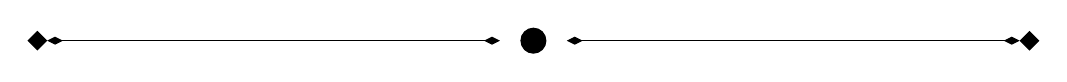
\begin{tikzpicture}[scale = 3]
		\node (a) at (0,0) {};
		\node (b) at (2,0) {};
		\draw[fill] (2.1, 0) circle (1.5pt);
		\node[draw, diamond, fill = black, scale = 0.5] at (0,0) {};
		\node (d) at (2.2,0) {};
		\node (e) at (4.2,0) {};
		\node[draw, diamond, fill = black, scale = 0.5] at (4.2,0) {};
		\draw [{Diamond}-{Diamond}] (a.east) -- (b.west);
		\draw [{Diamond}-{Diamond}] (d.east) -- (e.west);
	\end{tikzpicture}
\end{center}


\end{document}

